%-*-latex-*-
\sectionthree{Function call}
\begin{python0}
from solutions import *; clear()
\end{python0}

The runtime analysis for function call is similar when it comes to
computing the runtime of the \textit{body} of the function.
The only other things you need to be careful about are
\begin{enumerate}[nosep]
\item the cost of parameter passing
\item the cost of entering the function
\item the cost of returning from the function
\item the cost of return value
\end{enumerate}
(See CISS360 for details.
Also, see CISS240 note on functions, especially the function call stack.)
Here, cost means both time and memory.
You'll definitely need to know how to compute the cost for the case of
recursive functions.

Suppose you have a function \verb!f()!
that takes an array and returns the first value:
\begin{console}
int f(int x[])
{
    return x[0];
}
\end{console}
and \verb!main()! calls \verb!f()! like this:
\begin{console}
int main()
{
    int x[] = {1, 2, 3};
    // A. start timing
    int y = f(x);
    // B. end timing
    return 0;
}
\end{console}
What is the time taken (from point A to point B)?
Here's roughly what happens:
\begin{tightlist}
\item[1.] The arguments are stored somewhere (for instance in the function call stack). For this example, the address \verb!x! is stored.
\item[2.] The point of return from \verb!f()! is stored somewhere (for instance in the function call stack).
This means the address of the machine code to be executed after returning
is stored.
\item[3.] The \defone{program counter} is set to the address of \verb!f()!.
  The program counter is a device in the CPU that basically remembers
  the address of the machine code of your program to execute next.
\item[4.]
  Function \verb!f()! begins execution including
  creating parameters using the value(s) stored in the
  function call stack.
\item[5.] 
  If there is a return value, the function has to store
  the return value somewhere.
\item[6.]
  The program counter is set to the point of return from
  function call \verb!f()!.
\item[7.]
  \verb!main()! continues execution.
\end{tightlist}
(I said roughly because it's an over-simplification, but sufficient for us to
compute the time and space complexity.)

The time taken to set the program counter in order to enter \verb!f()! or return to
\verb!main()! is constant.
The time taken to store the point of return to \verb!main()! is also constant.
The space usage for address of the function and point of return is also constant.
So we don't really care too much about the above, time-wise or space-wise.
The main cost would be the time and space usage for
\begin{tightlist}
  \li storing the arguments
  \li retrieving the arguments and constructing the parameters
  \li storing return value
\end{tightlist}

In the case of our example
\begin{Verbatim}[frame=single,fontsize=\footnotesize]
int f(int x[])
{
    return x[0];
}
\end{Verbatim}
the argument is the address of an array.
The amount of memory used is constant.
So the time to store the address,
retrieving the address, setting the parameter \verb!x! to this address
are all constant.
\verb!x! is a pointer since, from CISS245, the above code is the same
as
\begin{Verbatim}[frame=single,fontsize=\footnotesize]
int f(int * const x)
{
    return x[0];
}
\end{Verbatim}
so \verb!x! is most likely a 64-bit pointer (or 32).
For sure it does not depend on the size of the array.
So that space complexity is constant too.
\verb!x!.
No matter large the array \verb!x! points to, \verb!x! consumes
64 bits.
That's why the time taken to set up \verb!x!
and the space usage of \verb!x! are all constant.
(Don't remember pointers?
You had better re-study your pointer notes from CISS245.)

Therefore the total runtime to execute \verb!f()! is $O(1)$
and the space complexity if also $O(1)$.

Now suppose I want to use a \verb!std::vector< int >! instead of an
integer array.
What will happen then?

If I do this:
\begin{console}
int f(const std::vector< int > & x)
{
    return x[0];
}
\end{console}
then all timing are the same as before except that we need to think about
the time for setting up \verb!x!.
In this case, \verb!x! is a reference, which (recall), is just like a pointer.
So the total runtime is still $O(1)$ and the space complexity is still $O(1)$.

Now come the trick question ... what about this:
\begin{console}
int f(const std::vector< int > x)
{
    return x[0];
}
\end{console}
or
\begin{console}
int f(std::vector< int > x)
{
    return x[0];
}
\end{console}
In this case, \verb!x! is a \verb!std::vector< int >! \textit{object} -- it is
not a reference and not a pointer.
If in \verb!main()!, I have
\begin{console}
int main()
{
    std::vector< int > y;
    ...
    std::cout << f(y) << '\n';
    ...
}
\end{console}
then the \verb!x! of \verb!f()! is a \textit{copy} of \verb!y! of \verb!main()!,
created through the
copy constructor of \verb!std::vector!.
If \verb!y! is a vector of $1000$ values, then it takes
a certain amount of time to set up \verb!x!,
which includes requesting memory for \verb!x! and
\textit{copying} the 1000 values of \verb!y! to \verb!x!.
And if \verb!y! is a vector of $1000000000$ values, then it
takes even more time to set up \verb!x!. 
Therefore the set up time for \verb!x! is actually $O(n)$
where $n$ is the size of \verb!y!.
Hence this algorithm has a total runtime of $O(n)$ and the space complexity is also
$O(n)$.

In the same way if you \textit{return} a value that is large in size, then the time
due to returning might not be $O(1)$.
For instance look at this:
\begin{console}
std::vector< int > f(std::vector< int > & v)
{
    return v;
}
\end{console}
In this case, the parameter set up time is $O(1)$ because \verb!v! is a reference.
But the return type is a \verb!std::vector< int >! value (not reference).
So the copy constructor is used to create a \verb!std::vector< int >! value
for returning
from the value \verb!v! references.
So hidden in the above code is a $O(n)$ runtime where $n$ is the
size of the vector that \verb!v! references
and the space complexity is also $O(n)$.

This explains why in CISS245,
for \lq\lq large" variables such as \verb!struct! variables or objects,
we always pass by pointer or pass by reference.
This is the same reason that an array parameter of a function
is actually a pointer:
\begin{console}
void f(int x[]) // same as void f(int * const x)
{
    return v
}
\end{console}
This was also mentioned in CISS245.

\newpage
%-*-latex-*-

\begin{ex} 
  \label{ex:prob-00}
  \tinysidebar{\debug{exercises/{disc-prob-28/question.tex}}}

  \solutionlink{sol:prob-00}
  \qed
\end{ex} 
\begin{python0}
from solutions import *
add(label="ex:prob-00",
    srcfilename='exercises/discrete-probability/prob-00/answer.tex') 
\end{python0}
 

\newpage
Now suppose you have a sequence of function calls where the first function
called is \verb!f()!:
\begin{Verbatim}[frame=single,fontsize=\footnotesize,numbers=left]
void j(double y)
{
     int c[30];
}
void i(int x[])
{
     int c[30];
}
void h(int x[], double y)
{
     int c[30];
     i(x);
}
double g(int x[])
{
    double y;
    int b[20];
    h(x, y);
    int d[40];
    j(y);
}
int f(int x[])
{
    int a[10];
    g(x)
    return 42;
}
\end{Verbatim}
The following is the function call graph:
%-*-latex-*-
\begin{center}
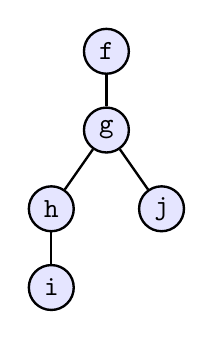
\begin{tikzpicture}

\fill[blue!10] (2.1, 0.0) circle (0.3);
\node [line width=0.03cm,black,minimum size=0.57cm,draw,circle] at (2.1,0.0)(f){};\draw (2.1, 0.0) node[color=black] {\texttt{f}};
\fill[blue!10] (2.1, -1.0) circle (0.3);
\node [line width=0.03cm,black,minimum size=0.57cm,draw,circle] at (2.1,-1.0)(g){};\draw (2.1, -1.0) node[color=black] {\texttt{g}};
\fill[blue!10] (1.4, -2.0) circle (0.3);
\node [line width=0.03cm,black,minimum size=0.57cm,draw,circle] at (1.4,-2.0)(h){};\draw (1.4, -2.0) node[color=black] {\texttt{h}};
\fill[blue!10] (1.4, -3.0) circle (0.3);
\node [line width=0.03cm,black,minimum size=0.57cm,draw,circle] at (1.4,-3.0)(i){};\draw (1.4, -3.0) node[color=black] {\texttt{i}};
\fill[blue!10] (2.8, -2.0) circle (0.3);
\node [line width=0.03cm,black,minimum size=0.57cm,draw,circle] at (2.8,-2.0)(j){};\draw (2.8, -2.0) node[color=black] {\texttt{j}};\draw[line width=0.03cm,black] (f) to  (g);
\draw[line width=0.03cm,black] (g) to  (h);
\draw[line width=0.03cm,black] (g) to  (j);
\draw[line width=0.03cm,black] (h) to  (i);
\end{tikzpicture}

\end{center}


The following lists memory usage (by line numbers) at various points
during the program execution:
\begin{align*}
  \text{end of line 24}&: \text{10 integers} \\
  \text{end of line 17}&: \text{30 integers, 1 pointer, 1 double} \\
  \text{end of line 11}&: \text{60 integers, 2 pointer, 2 double} \\
  \text{end of line 26}&: \text{10 integers}
\end{align*}
Recall (from CISS245) that this structure is called a tree where \verb!f! is called the root
of the tree.
We'll be studying trees in detail.

Note that the space usage grows \textit{and shrinks} with program execution since
\begin{enumerate}[nosep]
  \li
  memory used a local variable is reclaimed when this local variable
  goes out of scope
  \li
  memory used by a function is reclaimed when you exit a function
  \li 
  memory in the heap is reclaimed when you deallocate the memory
\end{enumerate}
However time usage only increases with program execution.
You can reuse memory, but you cannot reuse time!!!
To compute the worst case scenario of memory usage, i.e., maximum memory usage,
you would need to consider the
memory usage by
\begin{enumerate}[nosep]  
  \li \verb!f()!
  \li \verb!f()! , \verb!g()!, 
  \li \verb!f()! , \verb!g()!, \verb!h()!
  \li \verb!f()!, \verb!g()!, \verb!h()!, \verb!i()! and
  \li \verb!f()!, \verb!g()!, \verb!j()!
\end{enumerate}
in the function call graph:
%-*-latex-*-
\begin{center}
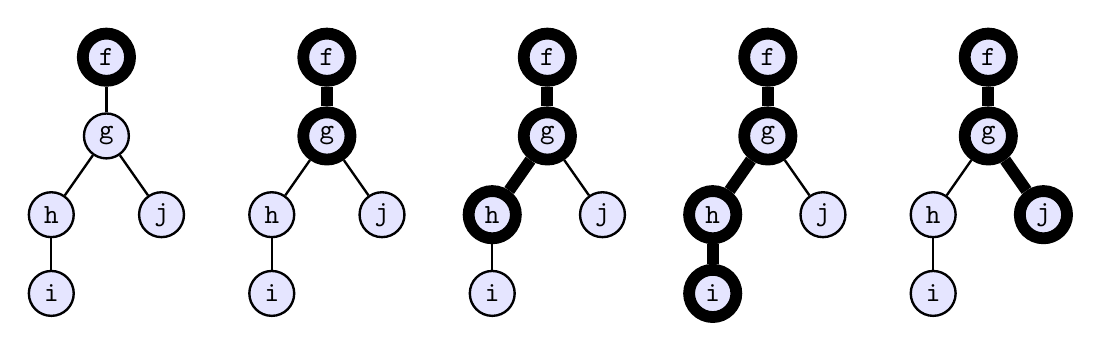
\begin{tikzpicture}

\fill[blue!10] (0.7, 0.0) circle (0.3);
\node [line width=0.15cm,black,minimum size=0.6cm,draw,circle] at (0.7,0.0)(A){};\draw (0.7, 0.0) node[color=black] {\texttt{f}};
\fill[blue!10] (0.7, -1.0) circle (0.3);
\node [line width=0.03cm,black,minimum size=0.57cm,draw,circle] at (0.7,-1.0)(B){};\draw (0.7, -1.0) node[color=black] {\texttt{g}};
\fill[blue!10] (0.0, -2.0) circle (0.3);
\node [line width=0.03cm,black,minimum size=0.57cm,draw,circle] at (0.0,-2.0)(C){};\draw (0.0, -2.0) node[color=black] {\texttt{h}};
\fill[blue!10] (0.0, -3.0) circle (0.3);
\node [line width=0.03cm,black,minimum size=0.57cm,draw,circle] at (0.0,-3.0)(D){};\draw (0.0, -3.0) node[color=black] {\texttt{i}};
\fill[blue!10] (1.4, -2.0) circle (0.3);
\node [line width=0.03cm,black,minimum size=0.57cm,draw,circle] at (1.4,-2.0)(E){};\draw (1.4, -2.0) node[color=black] {\texttt{j}};
\fill[blue!10] (9.1, 0.0) circle (0.3);
\node [line width=0.15cm,black,minimum size=0.6cm,draw,circle] at (9.1,0.0)(f){};\draw (9.1, 0.0) node[color=black] {\texttt{f}};
\fill[blue!10] (9.1, -1.0) circle (0.3);
\node [line width=0.15cm,black,minimum size=0.6cm,draw,circle] at (9.1,-1.0)(g){};\draw (9.1, -1.0) node[color=black] {\texttt{g}};
\fill[blue!10] (8.4, -2.0) circle (0.3);
\node [line width=0.15cm,black,minimum size=0.6cm,draw,circle] at (8.4,-2.0)(h){};\draw (8.4, -2.0) node[color=black] {\texttt{h}};
\fill[blue!10] (8.4, -3.0) circle (0.3);
\node [line width=0.15cm,black,minimum size=0.6cm,draw,circle] at (8.4,-3.0)(i){};\draw (8.4, -3.0) node[color=black] {\texttt{i}};
\fill[blue!10] (9.8, -2.0) circle (0.3);
\node [line width=0.03cm,black,minimum size=0.57cm,draw,circle] at (9.8,-2.0)(j){};\draw (9.8, -2.0) node[color=black] {\texttt{j}};
\fill[blue!10] (11.9, 0.0) circle (0.3);
\node [line width=0.15cm,black,minimum size=0.6cm,draw,circle] at (11.9,0.0)(F){};\draw (11.9, 0.0) node[color=black] {\texttt{f}};
\fill[blue!10] (11.9, -1.0) circle (0.3);
\node [line width=0.15cm,black,minimum size=0.6cm,draw,circle] at (11.9,-1.0)(G){};\draw (11.9, -1.0) node[color=black] {\texttt{g}};
\fill[blue!10] (11.2, -2.0) circle (0.3);
\node [line width=0.03cm,black,minimum size=0.57cm,draw,circle] at (11.2,-2.0)(H){};\draw (11.2, -2.0) node[color=black] {\texttt{h}};
\fill[blue!10] (11.2, -3.0) circle (0.3);
\node [line width=0.03cm,black,minimum size=0.57cm,draw,circle] at (11.2,-3.0)(I){};\draw (11.2, -3.0) node[color=black] {\texttt{i}};
\fill[blue!10] (12.6, -2.0) circle (0.3);
\node [line width=0.15cm,black,minimum size=0.6cm,draw,circle] at (12.6,-2.0)(J){};\draw (12.6, -2.0) node[color=black] {\texttt{j}};
\fill[blue!10] (3.5, 0.0) circle (0.3);
\node [line width=0.15cm,black,minimum size=0.6cm,draw,circle] at (3.5,0.0)(a){};\draw (3.5, 0.0) node[color=black] {\texttt{f}};
\fill[blue!10] (3.5, -1.0) circle (0.3);
\node [line width=0.15cm,black,minimum size=0.6cm,draw,circle] at (3.5,-1.0)(b){};\draw (3.5, -1.0) node[color=black] {\texttt{g}};
\fill[blue!10] (2.8, -2.0) circle (0.3);
\node [line width=0.03cm,black,minimum size=0.57cm,draw,circle] at (2.8,-2.0)(c){};\draw (2.8, -2.0) node[color=black] {\texttt{h}};
\fill[blue!10] (2.8, -3.0) circle (0.3);
\node [line width=0.03cm,black,minimum size=0.57cm,draw,circle] at (2.8,-3.0)(d){};\draw (2.8, -3.0) node[color=black] {\texttt{i}};
\fill[blue!10] (4.2, -2.0) circle (0.3);
\node [line width=0.03cm,black,minimum size=0.57cm,draw,circle] at (4.2,-2.0)(e){};\draw (4.2, -2.0) node[color=black] {\texttt{j}};
\fill[blue!10] (6.3, 0.0) circle (0.3);
\node [line width=0.15cm,black,minimum size=0.6cm,draw,circle] at (6.3,0.0)(V){};\draw (6.3, 0.0) node[color=black] {\texttt{f}};
\fill[blue!10] (6.3, -1.0) circle (0.3);
\node [line width=0.15cm,black,minimum size=0.6cm,draw,circle] at (6.3,-1.0)(W){};\draw (6.3, -1.0) node[color=black] {\texttt{g}};
\fill[blue!10] (5.6, -2.0) circle (0.3);
\node [line width=0.15cm,black,minimum size=0.6cm,draw,circle] at (5.6,-2.0)(X){};\draw (5.6, -2.0) node[color=black] {\texttt{h}};
\fill[blue!10] (5.6, -3.0) circle (0.3);
\node [line width=0.03cm,black,minimum size=0.57cm,draw,circle] at (5.6,-3.0)(Y){};\draw (5.6, -3.0) node[color=black] {\texttt{i}};
\fill[blue!10] (7.0, -2.0) circle (0.3);
\node [line width=0.03cm,black,minimum size=0.57cm,draw,circle] at (7.0,-2.0)(Z){};\draw (7.0, -2.0) node[color=black] {\texttt{j}};\draw[line width=0.03cm,black] (A) to  (B);
\draw[line width=0.03cm,black] (B) to  (C);
\draw[line width=0.03cm,black] (B) to  (E);
\draw[line width=0.03cm,black] (C) to  (D);
\draw[line width=0.15cm,black] (a) to  (b);
\draw[line width=0.03cm,black] (b) to  (c);
\draw[line width=0.03cm,black] (b) to  (e);
\draw[line width=0.03cm,black] (c) to  (d);
\draw[line width=0.15cm,black] (V) to  (W);
\draw[line width=0.15cm,black] (W) to  (X);
\draw[line width=0.03cm,black] (W) to  (Z);
\draw[line width=0.03cm,black] (X) to  (Y);
\draw[line width=0.15cm,black] (f) to  (g);
\draw[line width=0.15cm,black] (g) to  (h);
\draw[line width=0.03cm,black] (g) to  (j);
\draw[line width=0.15cm,black] (h) to  (i);
\draw[line width=0.15cm,black] (F) to  (G);
\draw[line width=0.03cm,black] (G) to  (H);
\draw[line width=0.15cm,black] (G) to  (J);
\draw[line width=0.03cm,black] (H) to  (I);
\end{tikzpicture}

\end{center}


For the case of computing runtime, you have to look at the time used
for \textit{all} functions:
%-*-latex-*-
\begin{center}
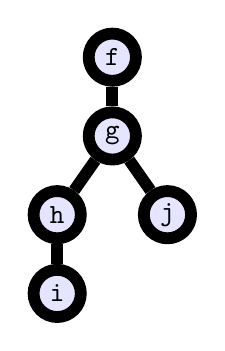
\begin{tikzpicture}

\fill[blue!10] (0.7, 0.0) circle (0.3);
\node [line width=0.15cm,black,minimum size=0.6cm,draw,circle] at (0.7,0.0)(A){};\draw (0.7, 0.0) node[color=black] {\texttt{f}};
\fill[blue!10] (0.7, -1.0) circle (0.3);
\node [line width=0.15cm,black,minimum size=0.6cm,draw,circle] at (0.7,-1.0)(B){};\draw (0.7, -1.0) node[color=black] {\texttt{g}};
\fill[blue!10] (0.0, -2.0) circle (0.3);
\node [line width=0.15cm,black,minimum size=0.6cm,draw,circle] at (0.0,-2.0)(C){};\draw (0.0, -2.0) node[color=black] {\texttt{h}};
\fill[blue!10] (0.0, -3.0) circle (0.3);
\node [line width=0.15cm,black,minimum size=0.6cm,draw,circle] at (0.0,-3.0)(D){};\draw (0.0, -3.0) node[color=black] {\texttt{i}};
\fill[blue!10] (1.4, -2.0) circle (0.3);
\node [line width=0.15cm,black,minimum size=0.6cm,draw,circle] at (1.4,-2.0)(E){};\draw (1.4, -2.0) node[color=black] {\texttt{j}};\draw[line width=0.15cm,black] (A) to  (B);
\draw[line width=0.15cm,black] (B) to  (C);
\draw[line width=0.15cm,black] (B) to  (E);
\draw[line width=0.15cm,black] (C) to  (D);
\end{tikzpicture}

\end{center}


and if \verb!g()! calls either \verb!h()! or \verb!j()! (but not both),
then you have to consider
\begin{enumerate}[nosep]  
  \li \verb!f()!, \verb!g()!, \verb!h()!, \verb!i()! and
  \li \verb!f()!, \verb!g()!, \verb!j()!
\end{enumerate}

Remember: you can reuse space, but you cannot reuse time!!!

\newpage%-*-latex-*-

\begin{ex} 
  \label{ex:prob-00}
  \tinysidebar{\debug{exercises/{disc-prob-28/question.tex}}}

  \solutionlink{sol:prob-00}
  \qed
\end{ex} 
\begin{python0}
from solutions import *
add(label="ex:prob-00",
    srcfilename='exercises/discrete-probability/prob-00/answer.tex') 
\end{python0}

\newpage%-*-latex-*-

\begin{ex} 
  \label{ex:prob-00}
  \tinysidebar{\debug{exercises/{disc-prob-28/question.tex}}}

  \solutionlink{sol:prob-00}
  \qed
\end{ex} 
\begin{python0}
from solutions import *
add(label="ex:prob-00",
    srcfilename='exercises/discrete-probability/prob-00/answer.tex') 
\end{python0}

\newpage%-*-latex-*-

\begin{ex} 
  \label{ex:prob-00}
  \tinysidebar{\debug{exercises/{disc-prob-28/question.tex}}}

  \solutionlink{sol:prob-00}
  \qed
\end{ex} 
\begin{python0}
from solutions import *
add(label="ex:prob-00",
    srcfilename='exercises/discrete-probability/prob-00/answer.tex') 
\end{python0}


%\newpage
%\subsection*{Solutions}
%
\newpage
\section*{Solutions}
Solution to Exercise \ref{ex:power-series-11}\labeltext{}{sol:power-series-11}.

\debug{\tinysidebar{exercises/{power-series-11/answer.tex}}}
 
(a) From
\begin{align*}
\sum_{n = 0}^\infty \frac{1}{2^n} x^n \cdot \sum_{n = 0}^\infty \frac{1}{2^n} x^n
&=
\left(
1 + \frac{1}{2}x + \frac{1}{4}x^2 + \frac{1}{8}x^3 + \cdots
\right)
\left(
1 + \frac{1}{2}x + \frac{1}{4}x^2 + \frac{1}{8}x^3 + \cdots
\right)
\end{align*}
the coefficient of $x^3$ is
\[
1 \cdot \frac{1}{8}
+ \frac{1}{2} \cdot \frac{1}{4}
+ \frac{1}{4} \cdot \frac{1}{2}
+ \frac{1}{8} \cdot 1
= 4 \cdot \frac{1}{8} = \frac{1}{2}
\]
The coefficient of $x^n$ is
\[
\sum_{k=0}^n \frac{1}{2^k} \cdot \frac{1}{2^{n-k}}
= \sum_{k=0}^n \frac{1}{2^k \cdot 2^{n-k}}
= \sum_{k=0}^n \frac{1}{2^n}
= \frac{n + 1}{2^n}
\]

(b)
First let's derive the coefficient of $x^n$ in general. 
The coefficient of $x^n$ is
\begin{align*}
\sum_{k=0}^n \frac{1}{2^k} \cdot \frac{1}{3^{n-k}}
&= \sum_{k=0}^n \frac{1}{2^k} \cdot \frac{3^k}{3^n} 
= \frac{1}{3^n} \sum_{k=0}^n \left(\frac{3}{2}\right)^k \\
&= \frac{1}{3^n} \cdot \frac{1 - (3/2)^{n+1}}{1 - 3/2} \\
&= \frac{1}{3^n} \cdot \frac{1 - (3/2)^{n+1}}{-1/2} \\
&= \frac{1}{3^n} \cdot \frac{(3/2)^{n+1} - 1}{1/2} \\
&= \frac{2}{3^n} \cdot \left( \frac{3^{n+1}}{2^{n+1}} - 1 \right) \\
&= 2 \cdot \left( \frac{3^{n+1} - 2^{n+1}}{2^{n+1}3^n} \right) \\
&= \frac{3^{n+1} - 2^{n+1}}{6^n}
\end{align*}
The coefficient of $x^3$ is
\[
\frac{3^4 - 2^{4}}{6^4} = \frac{65}{216}
\]



\newpage

Solution to Exercise \ref{ex:power-series-15}\labeltext{}{sol:power-series-15}.

\debug{\tinysidebar{exercises/{power-series-15/answer.tex}}}
We have
\begin{align*}
\left( \sum_{n=0}^\infty x^n \right)^{100} 
&= \left( \frac{1}{1 - x} \right)^{100} \\
&= \sum_{n=0}^\infty \binom{100 + n - 1}{n} x^n \\
&= \sum_{n=0}^\infty \binom{n + 99}{n} x^n \\
&= \sum_{n=0}^\infty \binom{n + 99}{99} x^n
\end{align*}
Hence the coefficient of $x^n$ is $\binom{n + 99}{99} x^n$ for $n \geq 0$.


\newpage

Solution to Exercise \ref{ex:power-series-16}\labeltext{}{sol:power-series-16}.

\debug{\tinysidebar{exercises/{power-series-16/answer.tex}}}

We have
\begin{align*}
&\left( 
2 + 5x + \frac{7}{1 - x}
\right)
\left( \sum_{n=0}^\infty x^n \right)^{100}
\\
&= \left( 
2 + 5x + \frac{7}{1 - x}
\right)
\left( \frac{1}{1 - x} \right)^{100}
\\
&=
2\left( \frac{1}{1 - x} \right)^{100}
+ 5x \left( \frac{1}{1 - x} \right)^{100}
+ \frac{7}{1 - x} \left( \frac{1}{1 - x} \right)^{100}
\\
&=
2 \sum_{n=0}^\infty \binom{100 + n - 1}{n} x^n
+ 5x \sum_{n=0}^\infty \binom{100 + n - 1}{n} x^n
+ 7 \left( \frac{1}{1 - x} \right)^{101} 
\\
&=
2 \sum_{n=0}^\infty \binom{n + 99}{n} x^n
+ 5x \sum_{n=0}^\infty \binom{n + 99}{n} x^n
+ 7 \sum_{n=0}^\infty \binom{101 + n - 1}{n}
\\
&=
\sum_{n=0}^\infty 2 \binom{n + 99}{99} x^n
+ \sum_{n=0}^\infty 5 \binom{n + 99}{99} x^{n+1}
+ \sum_{n=0}^\infty 7 \binom{n + 100}{n} x^n
\\
&=
\sum_{n=0}^\infty 2 \binom{n + 99}{99} x^n
+ \sum_{p=1}^\infty 5 \binom{p + 98}{99} x^{p}
+ \sum_{n=0}^\infty 7          \binom{n + 100}{n} x^n  \,\,\, \text{(let $p = n + 1$)}
\\
&=
\sum_{n=0}^\infty 2\binom{n + 99}{99} x^n
+ \sum_{n=1}^\infty 5 \binom{n + 98}{99} x^{n}  
+ \sum_{n=0}^\infty 7 \binom{n + 100}{100} x^n \,\,\,\text{(replace $p$ by $n$)}
\\
&=
2 \binom{99}{99} + \sum_{n=1}^\infty 2\binom{n + 99}{99} x^n
+ \sum_{n=1}^\infty 5\binom{n + 98}{99} x^{n} 
+ 7\binom{100}{100}  + \sum_{n=1}^\infty 7 \binom{n + 100}{100}  
\\
&=
9 +
\sum_{n=1}^\infty
\left( 2\binom{n + 99}{99} 
+  5\binom{n + 98}{99} 
+ 7 \binom{n + 100}{100}
\right) x^n
\end{align*}
Hence the coefficient of $x^n$ is
\[
\begin{cases}
9 & \text{ if } n = 0 \\
\displaystyle 2\binom{n + 99}{99} 
+  5\binom{n + 98}{99} 
+ 7 \binom{n + 100}{100} & \text{ if } n > 0
\end{cases}
\]


\newpage

Solution to Exercise \ref{ex:power-series-17}\labeltext{}{sol:power-series-17}.

\debug{\tinysidebar{exercises/{power-series-17/answer.tex}}}

(a)
\begin{align*}
\sum_{n=0}^\infty \frac{1}{2^n} x^n
\cdot
\sum_{n=0}^\infty \frac{1}{2^n} x^n
&=
\left( \sum_{n=0}^\infty \frac{1}{2^n} x^n \right)^2
\\
&=
\left( \sum_{n=0}^\infty \left( \frac{x}{2} \right)^n \right)^2
\\
&=
\left( \sum_{n=0}^\infty \left( \frac{x}{2} \right)^n \right)^2
\\
&=
\left( \frac{1}{1 - (x/2)} \right)^2
\\
&=\sum_{n=0}^\infty \binom{2 + n - 1}{n} \left( \frac{x}{2} \right)^n
\\
&=\sum_{n=0}^\infty \binom{n + 1}{n} \left( \frac{1}{2} \right)^n x^n
\\
\sum_{n=0}^\infty \left( \frac{n + 1}{2^n} \right x^n
\end{align*}

(b)
\begin{align*}
\sum_{n=0}^\infty \frac{1}{2^n} x^n
\cdot
\sum_{n=0}^\infty \frac{1}{3^n} x^n
\end{align*}
    


